\chapter{Diffusion Models for Surrogate Simulation}

Developing probabilistic generative models for physics data is a demanding yet fruitful task.
A major challenge posed by increasing collider experiment data is the computational resources required for detailed simulations.
Fast surrogate models can reduce the computational cost of event and detector simulation, can be used for template-based anomaly detection, or the inverse problem of unfolding.

One of the early objectives of this thesis was to develop a generative model specifically for collider data.
Unlike the data used in CV, it is inherently point-like, and unlike the data used in NLP, it is unordered and continuous.
These characteristics make physics data well suited to graphical representations, hence the success of GNNs models in jet tagging, as discussed in \Cref{ch:spice}.
Set generation methods, typically benchmarked on the ShapeNet dataset~\cite{ShapeNet}, provided a natural starting point for this work.

Other research groups had explored GNNs trained as GANs~\cite{MPGAN}, achieving some success but also encountered the typical drawbacks of GANs as detailed in \Cref{ch:generative_models}.
Our initial efforts focused on developing a graph-based VAE~\cite{SetVAE}, using a GNN decoder to transform pure noise into a reconstructed point cloud conditioned on the latent space.
While this approach worked on ShapeNet, it failed to generate high-quality samples of particle physics data.
The primary issue was identifying a suitable permutation-invariant loss term for reconstruction. Various attempts were made, including modifications to Sinkhorn~\cite{Sinkhorn}, Chamfer, and optimal transport losses, as well as physically motivated metrics specific to collider data~\cite{MetricSpaceCollider}, all yielding suboptimal results.

As diffusion models started to gain prominence, a realization was made that these models do not require permutation invariant losses as the training objective for diffusion models is denoising rather than generation.
This task is already permutation equivariant and thus could be achieved even using MSE, leading to the development of the first diffusion model for generating particle-type data.

This chapter summarizes a collection of work done to develop models for the conditional generation point cloud data, including particle physics jets~\cite{PCJedi, EpicJedi, PCDroid} and full events~\cite{PIPPIN}.
It also covers the use of these models for template-based anomaly detection~\cite{Drapes, RadOT}.

\section{\pcjedi}

An effective initial task for developing a generative model for collider data is generating individual particle physics jets.
These collimated showers of hadrons produce electrically charged and neutral particles within a cone originating from the interaction point.
Jet formation involves transitioning from perturbative QCD to a collection of colour-singlet hadrons, leptons, and photons.
While both regimes are well understood, the transition between them is not and continues to be a focal point of ongoing research.

Parton showers are typically constructed using a simple Markovian algorithm that stochastically transitions an $n$-parton state to an $(n+1)$-parton state.
This process is performed sequentially with dedicated generators such as \pythia~\cite{Pythia8}, \sherpa~\cite{Sherpa}, and \herwig~\cite{Herwig}.
These interactions with detector material are usually performed using \geant~\cite{Geant4}.
The high multiplicity of particles, the stochastic nature of showers, and their subsequent interaction with detector material make jets computationally expensive to simulate.
Fast parametric simulation tools such as \delphes~\cite{Delphes} are used to replace the computational expensive \geant in situations where computational resources are limited and the incurring a loss of detail is acceptable.

At the LHC, quarks can be produced in the decays of particles such as $W/Z$~bosons, or top quarks through their decay into a $W$~boson and a $b$-quark.
For the majority of energy scales the two or three quarks from these decays produce jets which can be individually resolved in the detector.
However, as the momenta of the intermediate particles increase, the decay products themselves start to collimate resulting in a single large-radius jet in the detector (the so-called boosted regime).
These objects are colloquially referred to as \textit{fat jets}.
The vast majority of jets, however, are initiated by partons which are not the decay products of other massive particles (QCD background).

Our first attempt to create a diffusion model for the these jets was called \pcjedi~\cite{PCJedi}\footnote{Code for this project is publicly available~\cite{PCJediCode}}.

\subsection{Diffusion Schedule}

\pcjedi was developed using the score matching diffusion framework from~\textcite{ScoreBasedGenerativeModeling} which is covered in \Cref{sec:score_based}.
We chose to use SM-TI schedule with hyperparameters $\sigma_\text{max}<1$ and $\sigma_\text{min}>0$, giving the following expressions for the signal and noise levels,
\begin{align}
  \lambda_a & = \arccos(\sigma_\text{max}), \\
  \lambda_b & = \arccos(\sigma_\text{min}), \\
  s(t) & = \cos\bigl(\lambda_a + t(\lambda_b - \lambda_a)\bigr), \\
  \sigma(t) & = \sin\bigl(\lambda_a + t(\lambda_b - \lambda_a)\bigr).
\end{align}
Following the derivation in \Cref{sec:score_based}, this results in the reverse SDE of the form,
\begin{equation}
    \label{eq:jedi_reverse_vp_sde}
    \diff\x_t = f(t) \left[ \x_t + 2 \score \right] \diff t + \sqrt{2 f(t)} \diff \bar\w_t,
\end{equation}
and the probability flow ODE,
\begin{equation}
    \label{eq:jedi_vp_ode}
    \diff \x_t = f(t) \left[ \x_t + \score \right] \diff t.
\end{equation}
Here $f(t)$ is related to the signal rate via,
\begin{equation}
    s(t) = \exp\left(\int_0^t f(s) \diff s\right),
\end{equation}
and solving this equation yields
\begin{equation}
    f(t) = (\lambda_b - \lambda_a) \tan\bigl(\lambda_a + t(\lambda_b - \lambda_a)\bigr).
\end{equation}

This task was framed using the standard SM objective, where a neural network is trained to predict the noise that was used to corrupt some data sample from \Cref{eq:noise_loss}.
The is extended for conditional generation based on context variable $\con$ and a hybrid loss term to give the training objective,
\begin{equation}
    \label{eq:training_objective}
    \mathcal{L}(\theta) =
    \E_{t\sim \mathcal{U}(0, 1)}
    \E_{\x_0, \con \sim \mathcal{D}},
    \E_{\z \sim \normal}
    \left(1 + \alpha \frac{4f(t)^2}{\sigma(t)^2}\right)
    \| \hat\e_\theta (\x_t, t, \con) - \e \|^2.
\end{equation}
The coefficient $\sfrac{4f(t)^2}{\sigma(t)^2}$ ensures that training corresponds to a maximum likelihood objective.
However, this can lead to unstable training, so many models in CV use the simple objective with no extra coefficient in front of the loss.
We use hyperparameter $\alpha$ to that controls the relative weight of these two tasks~\cite{ImprovedDenoisingDiffusion}.

\subsection{Data}
\label{sec:jetgen_data}

We used the open dataset JetNet30~\cite{MPGAN} in these experiments.
To construct this dataset, proton-proton collision events were simulated with a centre of mass energy $13~\TeV$ at leading order using \madgraph~\cite{MadGraph} and the \textsc{NNPDF2.3LO}~\cite{PDF2.3} set of parton distribution functions.
The transverse momenta of the partons and bosons were generated with $\pt \approx 1~\TeV$.
Showering was performed using \pythia 8.212~\cite{Pythia8} with the Monash tune~\cite{Monash}.
Jets were clustered using the anti-$k_T$ algorithm~\cite{AntiKt} with a distance parameter $R=0.8$ using \fastjet~\cite{FastJet} and were required to have reconstructed $0.8 < \pt < 1.6~\TeV$.
No detector simulation was performed.
Five classes of jets were simulated based on the initiating particle: top quark, $W$~boson, $Z$~boson, gluon, and light quark.
For each class, around 170k jets were produced with 50k of these reserved for evaluation.
For \pcjedi we only used the gluon and top quark datasets.

Each jet is characterized by a set of its constituents, often called the particle cloud.
These are the individual hadrons, leptons, and photons that were reconstructed and associated with the jet.
Only the leading 30 constituents in \pt were retained, and each constituent is effectively massless and is described solely by its momentum.

\subsubsection{Input and Conditional Features}

The task of the model was to generate the properties of the particle cloud given requested jet properties, specifically the net transverse momentum $\ptjet$ and invariant mass $\mjet$.
This conditional task is seen as a first step in developing a surrogate forward model for fast simulation.

Constituents are represented by the three kinematic variables $\left(\Delta\eta, \Delta\phi, \log(\pt + 1)\right)$.
The $\Delta\eta$ and $\Delta\phi$ are the differences in pseudorapidity and azimuthal angle between the constituent and the jet axis, and $\pt$ is the transverse momentum of the constituent.
We found that the log transformation of \pt ensured that the input distribution did not possess long tails, and this helped the generation of low-momentum constituents.
We used standard normalization techniques to scale the inputs and targets to zero mean and unit variance.

The model receives three inputs.
First is the set of noise-augmented constituents $\x_t$.
To construct these inputs, we sample a set of noise vectors $\z$ from a standard normal distribution matching the size of the constituent set.
This is added to the constituent kinematics with the signal and noise levels determined by the diffusion time parameter $t$.
The diffusion time parameter is itself sampled from a uniform distribution $\mathcal{U}(0, 1)$, and also passed to the model as an input.
Finally, the conditional jet variables $\con = (\ptjet, \mjet)$ are also provided as inputs.
The targets for the model is simply the set of noise vectors $\z$.

% \subsection{Evaluation Metrics}
% \label{sec:jetgen_eval}

% To evaluate the performance of the generative models in this section, we used distributional differences of specific observables between the generated and true jets.

% Included in this evaluation are the distributions of the generated constituent momentum values
% as well as several high level observables that are calculated from the particle cloud, these high level observables include the jet kinematics, and various substructure observables introduced in \Cref{sec:jet_substructure}.

% Beyond the observables in Ref.~\cite{MPGAN}, we analyze the jet $N$-subjettiness ratios $\tau_{32}$ and $\tau_{21}$, and the energy correlation function ratio $D_2$, which are crucial for identifying top jets and are strongly correlated with jet mass and transverse momentum. We study the two-dimensional marginals of these distributions and the invariant mass to assess the underlying correlations.

% To compare with MPGAN-generated jets, we calculate observables using the relative $\pt$ of constituents, defined as $\pt/p_\mathrm{T}^{\text{jet}}$ per constituent, denoted with the superscript `rel’. This rescaling tests the same underlying physics. For $N$-subjettiness ratios, the scale effects cancel out.

% We quantify distributional distances between MC and generated jets using the averaged Wasserstein-1 distance metric $\mathrm{W}_1$. Specifically, $\mathrm{W}1^M$ measures the distance between distributions of constituents' relative mass $m{j}^\text{rel}$, $\mathrm{W}_1^P$ the average distance between distributions of constituents' three momentum $(\Delta\eta, \Delta\phi, \pt^\text{rel})$, and $\mathrm{W}_1^{EFP}$ the average $\mathrm{W}_1$ using the first five EFPs. The distances for $N$-subjettiness ratios and $D_2$ are denoted $\mathrm{W}1^{\tau{32}}$, $\mathrm{W}1^{\tau{21}}$, and $\mathrm{W}_1^{D_2}$.

% Additionally, we compute the Fréchet ParticleNet distance (FPND)~\cite{MPGAN}, comparing the mean and standard deviation of the penultimate layer of the ParticleNet model for MC and generated jets~\cite{MPGAN, ParticleNet}. We also evaluate coverage (Cov) and minimum matching distance (MMD) metrics as described in Ref.~\cite{MPGAN}.

\subsection{Model Architecture}

A schematic overview of the \pcjedi model is shown in \Cref{fig:pcjedi}.
The inputs to the model includes the noisy set of jet constituents.
The training objective is to predict the noise vector added to each constituent, and is thus inherently permutation equivariant.
Therefore, so long as the model itself is permutation equivariant, we are able to use a basic loss for training.
An implicit conditional feature is therefore the number of constituents in the jet, which is built into the input data.

Our model comprised of four TE Blocks, each utilizing multi-headed self-attention.
We used blocks based architecture of ~\textcite{Normformer}.
An initial MLP embedded the three-dimensional noisy particle cloud into a larger space of 128 dimensions to enable expressive self-attention, while a MLP reshaped the output tokens back to the original dimension.
All MLPs in the model, including those within the TE Block, used the SiLU activation function, had a single hidden layer with 256 units followed by dropout with $p=0.1$ and layer normalization.
The diffusion time parameter was encoded using a CosEnc layer, described in \Cref{sec:time_encoding}, after which it was concatenated to the other conditional inputs $\ptjet$ and $\mjet$.
These combined context variables were concatenated to the input of every MLP in the model.

Fixed normalization layers using values derived from the entire training set ensured that the data distribution used in the diffusion process had zero mean and unit variance.
For the training objective, we found that using Huber loss instead of the Frobenius norm results in faster training and better generation quality.
We performed a scan over hyperparameters $\alpha$, $\sigma_\text{max}$, and $\sigma_\text{min}$, and found the best generative performance with $\alpha=10^{-3}$, $\sigma_\text{max}=0.999$, and $\sigma_\text{min}=0.02$.

We trained separate networks for generating the top quark and gluon jets in the dataset.
The Adam optimizer was used with default settings and a batch size of 256.
The learning rate ramped up linearly from 0 to $5 \times 10^{-4}$ over the first 10k training iterations.
Training ran for 100k iterations.
The network saved for evaluation was an exponential moving average (EMA) of the network with a decay rate of 0.999.

\begin{figure}
    \centering
    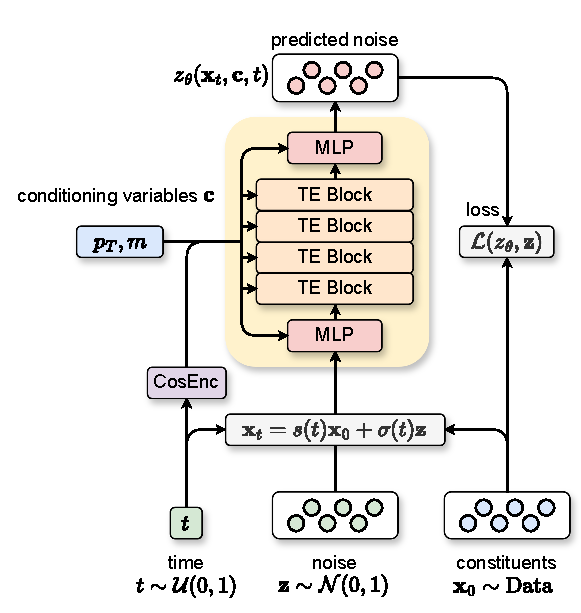
\includegraphics[width=0.5\textwidth]{Figures/jet_generation/pcjedi.pdf}
    \caption{The \pcjedi model architecture configured for training.}
    \label{fig:pcjedi}
\end{figure}

\subsection{Results}

To generate jets with \pcjedi, numerical integration is required to solve the reverse SDE or the probability flow ODE.
We compared various numerical solvers for this task~\cite{NumericalSolutionStochastic}.

The Euler-Maruyama (EM) method was used to solve the reverse SDE, and the standard Euler solver and fourth-order Runge-Kutta (RK) method~\cite{RungeKutta} were used for the probability-flow ODE.
Finally, the deterministic DDIM solver~\cite{DDIM}, designed for diffusion generative models was also used.
Generating higher quality jets requires more integration steps, increasing generation time as each step requires at least one forward pass through the model.
We focused on quality rather than speed, allowing for 200 forward passes, which corresponds to 50 integration steps for RK and 200 for EM, DDIM, and Euler.
Equal step sizes were used for all solvers.


First we focus on the inclusive generation of jets following the same $\pt^\text{jet}$ and $m_\mathrm{jet}$ distributions seen during training.
This allows us to compare directly to the non-conditional MPGAN model.%
\footnote{For fair comparisons we use the trained model provided by Ref.~\cite{MPGAN} and generate an equal number of jets with both \pcjedi and MPGAN and evaluate all metrics consistently for both models using the \texttt{JetNet} library provided with the datasets.}
For these comparisons we calculate the relative transverse momentum ($\pt^\text{rel}$) of each constituent using the full $\pt$ of the jet.
% This variable is labelled $\pt^\text{rel}$.
% Additional kinematic and substructure variables calculated using $\pt^\text{rel}$ in place of $\pt$ are denoted with superscript `rel'.

\begin{figure}[hbpt]
    \centering
    \includegraphics[width=.66\linewidth]{figures/gluon_generation/jet_features_rel.pdf}
    \caption{The relative transverse momentum (left) and invariant mass (right) of gluon jets generated with MPGAN (orange) and \pcjedi (DDIM solver, green; EM solver, red) compared to the MC simulation (shaded blue).
    Calculated from the leading 30 \pt constituents using the constituent $p_\mathrm{T}^\mathrm{rel}$ instead of $p_\mathrm{T}$.}
    \label{fig:kinematics_gluon}
\end{figure}

\begin{figure}[hbpt]
    \centering
    \includegraphics[width=.66\linewidth]{figures/top_generation/jet_features_rel.pdf}
    \caption{The relative transverse momentum (left) and invariant mass (right) of top jets generated with MPGAN (orange) and \pcjedi (DDIM solver, green; EM solver, red) compared to the MC simulation (shaded blue).
    Calculated from the leading 30 \pt constituents using the constituent $p_\mathrm{T}^\mathrm{rel}$ instead of $p_\mathrm{T}$.}
    \label{fig:kinematics_top}
\end{figure}

We look at the relative transverse momentum $\pt^{\text{rel}}$ and relative invariant mass $m_\mathrm{jet}^\text{rel}$ of the reconstructed jet.
These observables are calculated from the vector sum of the 30 (leading in \pt) jet constituents using $\pt^\text{rel}$ in place of $\pt$ per constituent.
These are shown in \cref{fig:kinematics_gluon,fig:kinematics_top} for gluon jets and top jets,   respectively.
The value of $\pt^\text{jet, rel}$ is not always exactly 1.0 due to selecting only the leading 30 constituents for each jet.
However this is the maximum physical value.
All generative models struggle to capture the hard cut off at 1.0 in $\pt^\text{jet, rel}$, though \pcjedi with the DDIM solver is closest in agreement.
Both \pcjedi models outperform MPGAN at reconstructing the top jet $\pt^\text{rel}$ distribution.
All three models perform similarly at reproducing the $m_\mathrm{jet}^{\text{rel}}$ for both top quarks and gluons.


It is also important that the individual constituents are accurately modelled.
In \cref{fig:gluon_const_pt,fig:top_const_pt} we see that the relative transverse momentum of the leading three constituents ordered by \pt are well reproduced by MPGAN and \pcjedi for both gluon and top jets.
However, both \pcjedi models show disagreements at low values of transverse momentum for gluon jets.
Here, MPGAN is better able to capture these values.
The relative $\eta$ and $\phi$ coordinates of the constituents are found to be in good agreement with the MC simulation for all three models.

\begin{figure}[hbpt]
    \begin{subfigure}{.33\textwidth}
        \centering
        \includegraphics[width=1.\linewidth]{figures/gluon_generation/const1_pt.pdf}
    \end{subfigure}%
    \begin{subfigure}{.33\textwidth}
        \centering
        \includegraphics[width=1.\linewidth]{figures/gluon_generation/const2_pt.pdf}
    \end{subfigure}%
    \begin{subfigure}{.33\textwidth}
        \centering
        \includegraphics[width=1.\linewidth]{figures/gluon_generation/const3_pt.pdf}
    \end{subfigure}% \\
    \caption{Distributions of the leading (left), subleading (middle) and third leading (right) constituent $\pt^\text{rel}$ for the gluon jets generated with MPGAN (orange) and \pcjedi (DDIM solver, green; EM solver, red) compared to the MC simulation.}
    \label{fig:gluon_const_pt}
\end{figure}

\begin{figure}[hbpt]
    \begin{subfigure}{.33\textwidth}
        \centering
        \includegraphics[width=1.\linewidth]{figures/top_generation/const1_pt.pdf}
    \end{subfigure}%
    \begin{subfigure}{.33\textwidth}
        \centering
        \includegraphics[width=1.\linewidth]{figures/top_generation/const2_pt.pdf}
    \end{subfigure}%
    \begin{subfigure}{.33\textwidth}
        \centering
        \includegraphics[width=1.\linewidth]{figures/top_generation/const3_pt.pdf}
    \end{subfigure}% \\
    \caption{Distributions of the leading (left), subleading (middle) and third leading (right) constituent $\pt^\text{rel}$ for the top jets generated with MPGAN (orange) and \pcjedi (DDIM solver, green; EM solver, red) compared to the MC simulation.}
    \label{fig:top_const_pt}
\end{figure}

Finally, we look at the relative $\tau_{21}$, $\tau_{32}$ and $D_{2}$ substructure observables in \cref{fig:substructure_gluon,fig:substructure_top}.
Both \pcjedi and MPGAN are able to capture the $D_2$ distributions, with MPGAN visually showing better agreement.
However all three models struggle to capture both $\tau_{21}$ and $\tau_{32}$ for gluon jets.
This is even more apparent for top jets, which have a bi-modal structure in all three observables.

\begin{figure}[hbpt]
    \centering
    \includegraphics[width=1.\linewidth]{figures/gluon_generation/jet_substructure_rel.pdf}
    \caption{Relative substructure distributions $\tau_{21}^{\text{rel}}$ (left), $\tau_{32}^{\text{rel}}$ (middle) and $D_{2}^{\text{rel}}$ (right) for gluon jets generated with MPGAN (orange) and \pcjedi (DDIM solver, green; EM solver, red) compared to the MC simulation.}
    \label{fig:substructure_gluon}
\end{figure}

\begin{figure}[hbpt]
    \centering
    \includegraphics[width=1.\linewidth]{figures/top_generation/jet_substructure_rel.pdf}
    \caption{Relative substructure distributions $\tau_{21}^{\text{rel}}$ (left), $\tau_{32}^{\text{rel}}$ (middle) and $D_{2}^{\text{rel}}$ (right) for top jets generated with MPGAN (orange) and \pcjedi (DDIM solver, green; EM solver, red) compared to the MC simulation.}
    \label{fig:substructure_top}
\end{figure}

The performance is compared quantitatively in \cref{tab:kansal_results} for the metrics introduced in Ref.~\cite{MPGAN} and \cref{tab:substructure_metrics} for the additional substructure distributions in \cref{fig:substructure_gluon,fig:substructure_top}.
For each metric we establish an ideal limit by comparing the training and test sets, which corresponds to the natural variation in the MC samples.
Following the procedure defined by Ref.~\cite{MPGAN} uncertainties for the Wasserstein based metrics are derived using bootstrap sampling, however we increase the number of bootstrapped batches from 5 to 40 to reduce the run to run variance.
The FPND metric requires the entire test set and does not use bootsrapping so we do not quote an uncertainty.

\pcjedi beats the current methods for several metrics and is competitive across several others for both gluon and top jet generation.
For top generation \pcjedi has a notably lower FPND and $\mathrm{W_1^{P}}$ scores than MPGAN yet performs worse in $\mathrm{W_1^{M}}$ and $\mathrm{W_1^{EFP}}$.
The metrics \textbf{Cov} and \textbf{MMD} are essentially saturated by all models, as they are in agreement with the upper limit defined by the natural variation in the MC samples.
Some of the values seem to be in tension with visual inspection.
Most notably, $\mathrm{W_1^{P}}$ for gluon jets suggests \pcjedi with the EM solver outperforms MPGAN, despite the observed underestimation at low values of $\pt^{\text{rel}}$ for the three leading constituent.
This shows the importance of studying a wide range of distributions, and highlights a potential limitation in using aggregated $\mathrm{W_1}$ distances.
It may also suggest that a metric more sensitive to the behaviour in tails of distributions could be beneficial, for example classifier-based weight approaches~\cite{Das:2023ktd}.

Capturing the correlations between jet substructure observables and the jet kinematics is also a key measure of performance.
Cuts on $\tau_{32}$ and $D_{2}$ are applied to distinguish top jets from gluon or quark jets in simple cut-based analyses~\cite{ATLAS:2018wis,CMS:2020poo}, with cut values are often derived as a function of the jet mass.
Similarly $\tau_{21}$ is important in $W$-jet identification.
\Cref{fig:gluon_correlations,fig:top_correlations} show the distributions of these observables alongside the two-dimensional marginals for \pcjedi with the EM solver and MPGAN.
For gluon jets, \pcjedi captures the correlations between features better than MPGAN.
For top jets, both MPGAN and \pcjedi capture the bi-modal structure of the top jets with MPGAN showing slightly better agreement.

\begin{figure}[hbpt]
    \begin{subfigure}{0.5\textwidth}
        \centering
        \includegraphics[width=1.\linewidth]{figures/gluon_generation/subspread_em_200_rel.pdf}
    \end{subfigure}%
    \begin{subfigure}{0.5\textwidth}
        \centering
        \includegraphics[width=1.\linewidth]{figures/gluon_generation/subspread_mpgan_rel.pdf}
    \end{subfigure}%//
    \caption{Mass and relative substructure distributions of the generated gluon jets using the EM solver for \pcjedi, and MPGAN. The diagonal consists of the marginals of the distributions. The off-diagonal elements are the joint distributions of the variables.}
    \label{fig:gluon_correlations}
\end{figure}

\begin{figure}[hbpt]
    \begin{subfigure}{0.5\textwidth}
        \centering
        \includegraphics[width=1.\linewidth]{figures/top_generation/subspread_em_200_rel.pdf}
    \end{subfigure}%
    \begin{subfigure}{0.5\textwidth}
        \centering
        \includegraphics[width=1.\linewidth]{figures/top_generation/subspread_mpgan_rel.pdf}
    \end{subfigure}%
    \caption{Mass and relative substructure distributions of the generated top jets using the EM solver for \pcjedi, and MPGAN. The diagonal consists of the marginals of the distributions. The off-diagonal elements are the joint distributions of the variables.}
    \label{fig:top_correlations}
\end{figure}



% \subsection{PC-Droid}

% \subsection{Epic Jedi}

% For conditional generation, the combined mass and transverse momentum of the point cloud $(\pt^\text{jet}, m_\mathrm{jet})$ are provided during training and generation, calculated from the four-momentum vectors of the selected jet constituents. Since this dataset only includes a subset of the original jet constituents, the true transverse momentum and invariant mass of jets with more than 30 constituents exceed $\pt^\text{jet}$ and $m_\mathrm{jet}$.\footnote{For fast surrogate model applications, the $p_{\mathrm{T}}$ and $m_\mathrm{jet}$ calculated from all constituents would be used, unrestricted to 30 constituents.} For fair comparison with MPGAN, we use the same training and test splits as in Ref.~\cite{MPGAN}.

% \section{Method}

% This work focuses on two models for conditionally generating fat jets: PC-Jedi~\cite{PCJedi} and PC-Droid~\cite{PCDroid}.
% \pcjedi was developed initially using the diffusion framework from~\textcite{ScoreBasedGenerativeModeling}, whereas PC-Droid was developed using the framework from \textcite{ElucidatingDesignSpace}.
% Both were conditional models which would generation the point cloud of jet constituents based on the high level jet kinematics, but for each type of

% \section{PC-Droid}

% \section{Anomaly Detection}

% \subsection{Conclusion}

